\begin{figure}[htbp]
\centering
% Thesis-wide categorical color palette
% Usage: % Thesis-wide categorical color palette
% Usage: % Thesis-wide categorical color palette
% Usage: \input{figures/palette} in any figure file
%
% Muted primary colors -- print-friendly, visually distinct.
% Inspired by Cooper Union's red/blue primaries, softened for
% academic figures. Use palA-palC for data series in scatter
% plots, line charts, bar charts, etc.

\definecolor{palA}{HTML}{1F77B4}   % Tableau blue
\definecolor{palB}{HTML}{D62728}   % Tableau red
\definecolor{palC}{HTML}{2CA02C}   % Tableau green
 in any figure file
%
% Muted primary colors -- print-friendly, visually distinct.
% Inspired by Cooper Union's red/blue primaries, softened for
% academic figures. Use palA-palC for data series in scatter
% plots, line charts, bar charts, etc.

\definecolor{palA}{HTML}{1F77B4}   % Tableau blue
\definecolor{palB}{HTML}{D62728}   % Tableau red
\definecolor{palC}{HTML}{2CA02C}   % Tableau green
 in any figure file
%
% Muted primary colors -- print-friendly, visually distinct.
% Inspired by Cooper Union's red/blue primaries, softened for
% academic figures. Use palA-palC for data series in scatter
% plots, line charts, bar charts, etc.

\definecolor{palA}{HTML}{1F77B4}   % Tableau blue
\definecolor{palB}{HTML}{D62728}   % Tableau red
\definecolor{palC}{HTML}{2CA02C}   % Tableau green

\definecolor{sprcomp}{HTML}{C2D4A8}

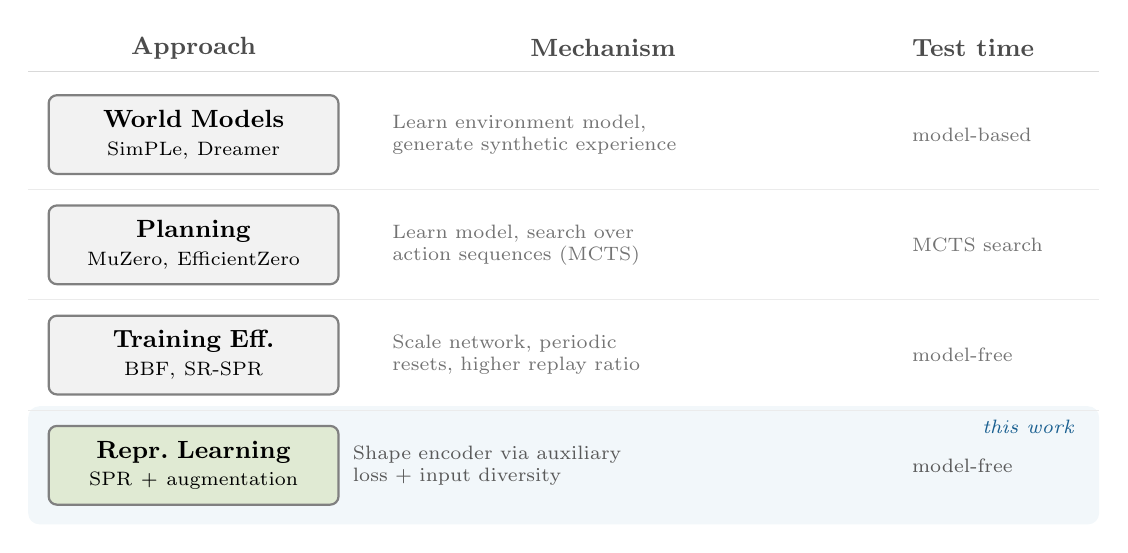
\begin{tikzpicture}[
    family/.style={draw=black!50, thick, rounded corners=3pt,
        minimum height=1.0cm, text width=3.4cm, align=center,
        font=\small, inner sep=4pt, fill=#1},
    mech/.style={font=\scriptsize, text=black!55, text width=3.8cm,
        align=left},
    ttime/.style={font=\scriptsize, text=black!55, anchor=west},
    heading/.style={font=\small\bfseries, text=black!70},
]

% === Column positions ===
\def\colA{0.3}     % Approach
\def\colB{5.5}     % Mechanism
\def\colC{10.2}    % Test time

% === Column headers ===
\node[heading] at (\colA, 0) {Approach};
\node[heading] at (\colB, 0) {Mechanism};
\node[heading] at (\colC, 0) {Test time};

% Divider line
\draw[black!15] (-1.8, -0.3) -- (11.8, -0.3);

% === Row 1: World Models ===
\def\rowA{-1.1}
\node[family=black!5] at (\colA, \rowA)
    {\textbf{World Models}\\[-1pt]
     {\scriptsize SimPLe, Dreamer}};
\node[mech, anchor=west] at (2.7, \rowA)
    {Learn environment model,\\
     generate synthetic experience};
\node[ttime] at (9.3, \rowA) {model-based};

% === Row 2: Planning ===
\def\rowB{-2.5}
\node[family=black!5] at (\colA, \rowB)
    {\textbf{Planning}\\[-1pt]
     {\scriptsize MuZero, EfficientZero}};
\node[mech, anchor=west] at (2.7, \rowB)
    {Learn model, search over\\
     action sequences (MCTS)};
\node[ttime] at (9.3, \rowB) {MCTS search};

% Row divider
\draw[black!8] (-1.8, -1.8) -- (11.8, -1.8);

% === Row 3: Training Efficiency ===
\def\rowC{-3.9}
\node[family=black!5] at (\colA, \rowC)
    {\textbf{Training Eff.}\\[-1pt]
     {\scriptsize BBF, SR-SPR}};
\node[mech, anchor=west] at (2.7, \rowC)
    {Scale network, periodic\\
     resets, higher replay ratio};
\node[ttime] at (9.3, \rowC) {model-free};

% Row divider
\draw[black!8] (-1.8, -3.2) -- (11.8, -3.2);

% === Row 4: This work (highlighted) ===
\def\rowD{-5.3}
\fill[palA!6, rounded corners=4pt]
    (-1.8, -4.55) rectangle (11.8, -6.05);

\node[family=sprcomp!50] at (\colA, \rowD)
    {\textbf{Repr.\ Learning}\\[-1pt]
     {\scriptsize SPR + augmentation}};
\node[mech, anchor=west, text=black!65] at (2.2, \rowD)
    {Shape encoder via auxiliary\\
     loss + input diversity};
\node[ttime, text=black!65] at (9.3, \rowD) {model-free};

% "This work" marker
\node[font=\scriptsize\itshape, text=palA!80!black,
    anchor=north east] at (11.6, -4.6) {this work};

% Row divider
\draw[black!8] (-1.8, -4.6) -- (11.8, -4.6);

\end{tikzpicture}
\caption{Data-efficient RL approaches. Each family addresses the
  limited-data problem through a different mechanism. This work
  studies representation learning in isolation -- the only approach
  that shapes the encoder without adding test-time computation or
  model-based planning.}
\label{fig:method-landscape}
\end{figure}
